\documentclass[12pt]{article}

% math
\usepackage{amsmath,amssymb}
\usepackage{eqnarray} % (deprecated, but retained in case you use it)
\usepackage{cancel}
\usepackage{algorithm}
\usepackage{algpseudocode}
\usepackage{bm}
\usepackage{syllogism}

% font
%\usepackage{fourier}
\usepackage[T1]{fontenc}
\usepackage{mathpazo,mathabx}
\usepackage[dvipsnames]{xcolor}

% headings
\usepackage{sectsty}
\sectionfont{\fontsize{12}{15}\selectfont}
\subsectionfont{\normalfont\fontsize{12}{15}\selectfont}
\subsubsectionfont{\itshape\normalfont\fontsize{12}{15}\selectfont}

% line numbers
\usepackage{lineno}

% footnotes
\usepackage[symbol]{footmisc}

% expectation operator
\usepackage{relsize}
\newcommand{\E}{\mathop{\vcenter{\hbox{\relsize{+1}$E$}}}}

% logit / expit operators
\DeclareMathOperator{\logit}{logit}
\DeclareMathOperator{\expit}{expit}

\newcommand{\Pn}{\mathbb{P}_n}

% accents (double hat)
\usepackage{accents}
\newlength{\dhatheight}
\newcommand{\doublehat}[1]{%
    \settoheight{\dhatheight}{\ensuremath{\hat{#1}}}%
    \addtolength{\dhatheight}{-0.15ex}%
    \hat{\vphantom{\rule{1pt}{\dhatheight}}%
    \smash{\hat{#1}}}}

% independence symbol
\newcommand{\bigCI}{\mathrel{\text{\scalebox{1.07}{$\perp\mkern-10mu\perp$}}}}

% lineno patch for amsmath envs
\newcommand*\patchAmsMathEnvironmentForLineno[1]{%
	\expandafter\let\csname old#1\expandafter\endcsname\csname #1\endcsname
	\expandafter\let\csname oldend#1\expandafter\endcsname\csname end#1\endcsname
	\renewenvironment{#1}%
	{\linenomath\csname old#1\endcsname}%
	{\csname oldend#1\endcsname\endlinenomath}%
}
\newcommand*\patchBothAmsMathEnvironmentsForLineno[1]{%
	\patchAmsMathEnvironmentForLineno{#1}%
	\patchAmsMathEnvironmentForLineno{#1*}%
}
\AtBeginDocument{%
	\patchBothAmsMathEnvironmentsForLineno{equation}%
	\patchBothAmsMathEnvironmentsForLineno{align}%
	\patchBothAmsMathEnvironmentsForLineno{flalign}%
	\patchBothAmsMathEnvironmentsForLineno{alignat}%
	\patchBothAmsMathEnvironmentsForLineno{gather}%
	\patchBothAmsMathEnvironmentsForLineno{multline}%
}

% misc
\usepackage{color}
\usepackage{wrapfig}
\usepackage{indentfirst}
\usepackage{setspace}
\usepackage[numbers,super,sort&compress]{natbib}
\usepackage{booktabs}
\usepackage{rotating}
\usepackage[margin = .85in]{geometry}
\usepackage{fancyhdr}
\pagestyle{fancy}
\fancyhf{}
%\renewcommand{\headrulewidth}{0pt}
\rfoot{\thepage}
\pagenumbering{arabic}
\usepackage{tabularx}
\usepackage{pdfpages}
\usepackage{longtable}
\usepackage{multirow}
\usepackage{multicol}
\usepackage{float}
\usepackage{lscape}
\usepackage{graphicx}
\usepackage{mdwlist}
\usepackage{url}
\urlstyle{same}
\usepackage{comment}
\usepackage{amsthm}

% figures and captions: use caption + subcaption (clean with hyperref)
\usepackage{caption}
\usepackage{subcaption}
%\captionsetup[sub]{position=top, font=large} % (replaces [subfloat] key)

% titlesec (kept as requested)
\usepackage[compact]{titlesec}

% remove square brackets in bib
\makeatletter
\renewcommand\@biblabel[1]{#1.}
\makeatother

\newtheorem*{remark}{Remark} % Unnumbered

% hyperlinks LAST (after most packages and natbib)
\usepackage[colorlinks=true, urlcolor=blue, linkcolor=black, citecolor=black]{hyperref}

% path to images
\graphicspath{{../figures/}}

\rhead{\color{red} Draft in progress}

\begin{document}
%%%%%%%%%%%%%%%%%%%%%%%%%%%%%%%%%%%%%%%%%%%%%%%%%%%%%%%%%%%%%%%%%%%%%%%%
\thispagestyle{empty}
\baselineskip=28pt

\noindent

\vskip 0.2cm {{\noindent \huge Residual-on-Residual Regression as a Tool for Analyzing Observational Data}}

\baselineskip=12pt

\vskip .25cm
\noindent Ashley I. Naimi, PhD$^{1,2 *}$\\[.5em]
\noindent Qianhui Jin, MPH$^{3}$\\[.5em]
\noindent Ya-Hui Yu, PhD$^{1}$\\[.5em]
\noindent Sara M Parisi, MPH$^{3}$\\[.5em]
\noindent Lisa M. Bodnar, PhD$^{3}$\\[.5em]

\vskip .25cm
\noindent $^1$ Department of Epidemiology, Emory University.\\[.5em]
\noindent $^2$ Department of Data and Decision Science, Emory University.\\[.5em]
\noindent $^3$ Department of Epidemiology, University of Pittsburgh.\\[.5em]

\vskip .25cm
\noindent \hskip -.2cm
\begin{tabular}{ll}
*Correspondence: & Department of Epidemiology \\[-.1cm]
& Rollins School of Public Health \\[-.1cm]
& Emory University \\[-.1cm]
& 1518 Clifton Road \\[-.1cm]
& Atlanta, GA 30322\\[-.1cm]
& \href{mailto:ashley.naimi@emory.edu}{ashley.naimi@emory.edu}
\end{tabular}

\vskip .25cm
\noindent Conflicts: The authors have no conflicts to disclose.
\vskip .25cm
\noindent Acknowledgements: We thank Dr Brian Whitcomb for comments on a previous version of this manuscript.
\vskip .25cm
\noindent Funding: This study is supported by grant funding from the National Institutes of Health: R01 HD102313 and R01 HL174652 to Naimi AI and Bodnar LM. The study sponsor had no role in the study design; collection, analysis, and interpretation of data; writing the report; or the decision to submit the report for publication.

\vskip .25cm
\vfill
\noindent \hskip -.2cm
\begin{tabular}{ll}
Target Journal: 	   & \emph{American Journal of Epidemiology} (Practice of Epidemiology) \\[-.01cm]
Text word count: 	   & / 4{,}000 \\[-.01cm]
Abstract word count:   & \\[-.01cm]
Number of Figures: 	   & 1 \\[-.01cm]
Number of Tables:      & 1 \\[-.01cm]
Number of References:  & 29 \\[-.01cm]
Running head:  & Residual on Residual Regression  \\
\end{tabular}
%
%
%%%%%%%%%%%%%%%%%%%%%%%%%%%%%%%%%%%%%%%%%%%%%%%%%%%%%%%%%%%%%%%%%%%%%%%%
\newpage
\thispagestyle{empty}
\begin{center}
{\Large{\bf Abstract}}
\\ To be written.
\end{center}
\baselineskip=12pt

\noindent

%%%%%%%%%%%%%%%%%%%%%%%%%%%%%%%%%%%%%%%%%%%%%%%%%%%%%%%%%%%%%%%%%%%%%%%%
%
%
%
\baselineskip=12pt
\par\vfill\noindent
{\bf KEY WORDS:} \\

%{\bf KEY MESSAGES}:
%\begin{itemize}
%	\item
%	\item
%	\item
%\end{itemize}
\par\medskip\noindent
%
%
%
%
%
%
%
%
%
%
%
%
%
%
%
%
%
%
%
%
%
%
%
%
%
\newpage
\doublespacing
%\linenumbers
\setcounter{page}{1}

\section{Introduction}

Researchers routinely use observational data to estimate confounder-adjusted causal effects of an exposure on an outcome of interest. Under key conditions for causal identification,\cite{Naimi2023a} several approaches can be deployed for effect estimation. When standard parametric regression models are used, researchers must correctly specify the functional form of the relationships between confounders and the outcome, and determine which confounder interactions should be included.\cite{Naimi2020a,Vansteelandt2022} In simple settings, when functional forms and relevant interactions might be known with some degree of confidence, standard parametric regression is a viable approach to estimating causal effects. However, causal effect estimation is regularly carried out with high-dimensional observational data, where the number of potential confounders is large relative to the sample size.\cite{Mitra2022} In such settings, correct functional form and interaction specification decisions can be difficult to make correctly. When misspecified, these models and estimators can introduce biases that standard sensitivity analyses may not detect.\cite{Naimi2023,Zivich2021}

Machine learning algorithms offer a data-adaptive alternative, capable of flexibly modeling complex confounder-confounder and confounder-exposure interactions without requiring functional forms to be pre-specified or known. Several machine learning algorithms are available to do this,\cite{Hastie2009} including ensemble learners such as the Super Learner, which optimally combines predictions from a library of candidate algorithms.\cite{Laan2007} However, most machine learning methods either implicitly or explicitly optimize a loss-function with respect to a bias-variance tradeoff between the observed and predicted outcomes (e.g., mean squared error). This can induce bias in the estimator for a target causal parameter, such as the average treatment effect. The resulting machine learning estimator of the target causal parameter inherits statistical properties that are not optimal, including slow convergence, estimation bias, biased standard errors, and less than nominal confidence interval coverage.\cite{Kennedy2024, Diaz2020} 

Fortunately, optimal statistical properties and valid statistical inference can be recovered by deriving estimators within a semiparametric efficiency theory, specifically, estimators built around Neyman-orthogonal scores or influence functions of pathwise differentiable causal estimands, which render the target parameter less sensitive to so-called ``first-order'' errors in nuisance estimation.\cite{Chen2026} The two approaches most widely used are augmented inverse probability weighting (AIPW)\cite{Robins1994} and targeted maximum likelihood estimation (TMLE).\cite{vanderLaan2006} Both are ``doubly robust'' in that they yield consistent estimates of the average treatment effect if at least one of the two nuisance functions (e.g., the outcome or propensity score model) is consistently estimated. When paired with some form of out-of-sample validation such as cross-fitting or cross-validation, both estimators achieve the nonparametric efficiency bound and support valid asymptotic inference.\cite{Kennedy2024}

However, these estimators are not a panacea for effect estimation. For instance, they can be particularly sensitive to even minor violations of the positivity assumption,\cite{Rudolph2022} which can occur when the sample size is not large enough to populate all confounder strata with exposed and unexposed individuals.\cite{Westreich2010,Petersen2012} For example, in nutritional epidemiology, researchers will often be interested in the effects of ``healthy'' dietary interventions (such as consuming enough vegetables per 1,000 kcals of diet to meet federally recommended guidelines) while adjusting for a large and complex set of confounding variables. Yet few people tend to meet dietary guidelines for vegetable consumption,\cite{Bodnar2023a} leading to questionable positivity for the desired estimand. Additionally, even when positivity is met, applying both TMLE and AIPW to the same data can yield different results, leading to uncertainty about which of the two estimates to rely on.

A less commonly used alternative to estimating causal effects with machine learning methods is a residual-on-residual approach, first introduced by Robinson in the late 1980s,\cite{Robinson1988} and more recently popularized in econometrics.\cite{Chernozhukov2018} Like AIPW and TMLE, it combines estimates of both outcome and exposure nuisance models. The approach is based on the specification of a partially linear model that encodes an average treatment effect under key assumptions.\cite{Robinson1988} It is particularly straightforward to implement and offers properties that complement those of AIPW and TMLE. Here, we illustrate residual-on-residual regression, provide R and Python code to reproduce all results, and discuss key assumptions, strengths, and limitations of the residual-on-residual regression approach as a tool for estimating causal effects.

\section{Methods}

\subsection{Data Source}

We used data from the Nulliparous Pregnancy Outcomes Study: Monitoring Mothers-to-Be (nuMoM2b), a U.S.-based pregnancy cohort study conducted across eight clinical centers (2010 to 2013).\cite{Haas2016} A total of 10,038 nulliparous pregnant individuals (no prior pregnancy $\geq$20 weeks of gestation) with singleton pregnancies were enrolled at 6 to 13 weeks' gestation. At enrollment, trained research staff administered questionnaires on periconceptional diet, medical history, and demographic, psychosocial, behavioral, and environmental factors. Medical records were reviewed $\geq$ 30 days after delivery to obtain information on pregnancy and birth outcomes. All participants provided written informed consent, and institutional review boards at each site approved the protocol. The final analytic cohort included 7,923 participants after excluding 2,115 (21\%) with missing dietary data.

\subsection{Exposure}

At enrollment, participants completed a self-administered food frequency questionnaire (FFQ), described previously,\cite{Bodnar2024,Bodnar2023b} to assess usual dietary intake (both frequency and portion size) during the three-month periconceptional period. Details are provided elsewhere.\cite{Bodnar2023b} We used data from the FFQ to construct our exposure, defined as {\color{OliveGreen} [Qianhui, what does v\_dich represent?]}.

\subsection{Outcome}

We defined preeclampsia using the 2013 American College of Obstetricians and Gynecologists' diagnostic criteria,\cite{ACOG2019} adapted by the nuMoM2b investigators to the data collected.\cite{Facco2017} Cases were identified as having 1) new-onset gestational hypertension (systolic blood pressure $\geq$ 140 or diastolic blood pressure $\geq$ 90 on 2 occasions $\geq$ 6 h apart or 1 occasion with subsequent antihypertensive therapy, excluding blood pressures recorded during the second stage of labor), and 2) 1 or more of the following and/or HELLP syndrome: proteinuria $\geq$ 300 mg/24 h; protein/creatinine ratio $\geq$ 0.3; or if other measures are not available, dipstick $\geq$ 1+, thrombocytopenia (platelet count $<$100,000/mm$^3$), pulmonary edema, serum creatinine $>$1.1 mg/dL, severe headache, scotoma, serum AST $\geq$ 100 IU/L, and epigastric pain.\cite{ACOG2019}

\subsection{Covariates}

Participants self-reported sociodemographic characteristics including age, education, race / ethnicity, marital status, public insurance status, nativity, English language proficiency, acculturation, and partner's education. Racial / ethnic identity had four mutually exclusive groups and was used as a proxy for exposure to structural racism.\cite{Ukoha2022} Income was assessed as a percentage of the federal poverty level. Prepregnancy BMI was calculated from self-reported prepregnancy weight and measured height at enrollment. Gravidity and whether the pregnancy was planned were self-reported. Pre-existing medical conditions including chronic hypertension, diabetes, sleep apnea risk, and thyroid medication use were ascertained from medical records. Standardized assessment tools\cite{Haas2015} measured depressive symptoms (Edinburgh Postnatal Depression Scale), perceived stress, anxiety, average nightly sleep duration, insomnia severity, and sleep satisfaction during the first trimester; nausea and vomiting severity was assessed using the Pregnancy Unique Quantification of Emesis (PUQE) score. Prepregnancy smoking status, alcohol use during pregnancy, and weekly alcohol consumption in the three months before pregnancy were self-reported. Physical activity in the 4 weeks before enrollment was assessed as total metabolic-equivalent task (MET) minutes per week.\cite{Piercy2018} Neighborhood characteristics such as the percentage of residents living below the federal poverty line, distance to nearby grocery stores, neighborhood walkability,\cite{Walker2013} and the area deprivation index,\cite{Kind2018} were derived from U.S. Census data linked to each participant's residential census tract and block group at enrollment. To account for the multidimensional nature of dietary patterns, overall diet quality was captured by the Healthy Eating Index 2010 (HEI-2010) total score, computed from the same food frequency questionnaire used to measure vegetable intake. Study site was included to account for potential between-center differences.

\subsection{AIPW and TMLE}

We first use AIPW and TMLE to estimate the average treatment effect, which can be encoded as a parameter in a nonparametric model:
\begin{equation}
Y = \mu(A, W) + \epsilon \label{eqn:nonpar}
\end{equation}
where $\mu(\bullet)$ is some nonparametric function, and where $E(\epsilon) = 0$. Throughout, we use $O = \{Y, A, W\}$ to denote the observed data, with outcome $Y$, exposure $A$, and confounding set $W$. Under standard causal identification assumptions,\cite{Naimi2023a} this model implies:
$$\psi = E[Y^{a = 1} - Y^{a = 0}] = E[\mu(A = 1, W) - \mu(A = 0, W)]$$
where $Y^{a}$ is the outcome that would be observed if $A$ were set to some value $a$. The right hand side of this equation is sometimes used as a plug-in estimator, and referred to as the g computation algorithm,\cite{Robins1986} or marginal standardization,\cite{Naimi2020,Muller2014} for a time-fixed exposure. Because $\psi$ is pathwise differentiable, its efficient influence function exists, and can be used to construct an equation that is a function of the observed data and the parameter $\psi$, and that equals zero when the parameter $\psi$ is set to the true value (i.e., an estimating equation).\cite{Ross2024} Solving the empirical analog of this estimating equation with nuisance functions fit to the data yields a regular, asymptotically linear estimator with variance equal to the semiparametric efficiency bound.\cite{Kennedy2024}

AIPW solves this estimating equation by augmenting the simple plug-in estimator with inverse-probability weights from an exposure model, a correction that removes first-order bias due to errors in either nuisance estimate.\cite{Kennedy2024} In contrast, TMLE is a substitution estimator that reaches the same solution indirectly, by tilting the initial outcome model predictions through a targeted fluctuation step parameterized by the propensity score model fit, until the estimating equation is satisfied, then plugs the updated predictions into the g-computation formula for $\psi$.\cite{Luque-Fernandez2018} Both AIPW and TMLE are well established methods extensively used in epidemiology.

\subsection{Residual-on-Residual Regression in a Partially Linear Model}

In contrast, residual-on-residual regression is less commonly deployed, though it shares some of the same doubly robust properties as AIPW and TMLE. Consider observed data on an outcome $Y$, exposure $A$, and a vector of measured confounders. We can define an effect of $A$ on $Y$ in the context of a \emph{partially} linear model such as:
\begin{equation}
Y = \psi A + g(C) + \epsilon \label{eqn:plm}
\end{equation}

In this equation, we use $g(C)$ to denote how the confounders relate to the mean of the outcome to account for the fact that we don't know the true relationship. This model is ``partially linear'' because it assumes that the exposure-outcome relationship is linear, but no such assumptions are made for the confounder-outcome relationships. Indeed, under this model, the confounder-outcome relationships can be linear, polynomial, logarithmic, or any other smooth function. This model is flexible in that it makes few assumptions about functional form, which lowers the chances of bias that results from model misspecification.

\subsection{The Intuition Behind Residual-on-Residual Regression}

Robinson first introduced a strategy to flexibly estimate $\psi$ encoded in this partially linear model.\cite{Robinson1988} His insight was based on the the notion that, if we could remove the influence of the confounders $C$ from both $Y$ and $A$, we could then estimate $\psi$ by regressing the ``de-influenced'' $Y$ on the ``de-influenced'' $A$. The challenge is how to remove $C$'s influence without knowing the functional form of that influence? Robinson showed that it is possible to eliminate $g(C)$ altogether in equation \ref{eqn:plm} if we use outcome and exposure residuals in a simple linear model:
\begin{equation}
Y - E[Y \mid C] = \psi \big( A - E[A \mid C] \big) + \epsilon \label{eqn:ronr}
\end{equation}

\noindent where $E[Y \mid C]$ and $E[A \mid C]$ are models regressing $Y$ against $C$, and $A$ against $C$. At face value, this procedure seems to simply transfer the problem from equation \ref{eqn:plm} to the fits for these models. However, Robinson's main contribution was to show that we can estimate these models nonparametrically, for example, using flexible machine learning methods, and still obtain a residual-on-residual estimator of $\psi$ using standard OLS with optimal statistical properties.

The residual-on-residual regression approach proceeds in three steps. The first is to estimate a model regressing $Y$ on only confounders $C$ (no exposure). Using nonparametric regression, such as a stacking algorithm like the super learner, estimate the conditional mean of $Y$ given $C$. Denote the predictions from this model $\hat{m}_Y(C)$, and use them to compute the residuals: $\tilde{Y} = Y - \hat{m}_Y(C)$. Do the same for the exposure, fitting a regression model for $E[A \mid C]$, construct residuals $\tilde{A} = A - \hat{m}_A(C)$. Once these residuals are constructed, the next step is to estimate $\psi$ using a no-intercept ordinary least squares estimator regressing $\tilde{Y}$ against $\tilde{A}$. The resulting estimator is consistent and asymptotically normal, with optimal statistical properties despite using machine learning to estimate $\hat{m}_Y(C)$ and $\hat{m}_A(C)$.

\subsection{Out-of-Sample Validation}

While residual-on-residual regression improves upon na\"{i}ve use of machine learning to estimate $\psi$, its performance can should be improved further still using some form of out-of-sample validation,\cite{Zivich2022} including sample splitting, cross fitting, or cross validation. The simplest approach is to use cross-validation when fitting models for $m_Y(C)$ and $m_A(C)$. Importantly, the same individuals in each fold are used to train both algorithms. This creates a set of $K$ folds, each with predictions for $\hat{m}_Y(C)$ and $\hat{m}_A(C)$. Once created, these $K$ test folds can be combined back into a single dataset, residuals constructed, and the no-intercept OLS deployed.

\section{Application to NuMoM2b Data}

We applied residual-on-residual regression, AIPW, and TMLE to estimate the association between high vegetable intake ($\geq$ 1.25 cups per 1{,}000 kcal) and the risk of preeclampsia defined according to the American College of Obstetricians and Gynecologists' diagnostic criteria. We used data from 7{,}923 participants in the Nulliparous Pregnancy Outcomes Study: Monitoring Mothers-to-Be (nuMoM2b) who had complete exposure and outcome data. We adjusted for potential confounders including age, education, race / ethnicity, medical insurance, prepregnancy smoking, and prepregnancy body mass index (BMI). Missing confounders were addressed using mean or mode imputation with indicators for missingness included in the models. Exposure and outcome models were estimated using a 10-fold cross-fitted Super Learner ensemble, which included the sample mean, generalized linear models, random forests (ranger), regularized regression using the elastic net (glmnet), and multivariate adaptive regression splines (earth).

Among participants, 2{,}045 (25.8\%) had high vegetable intake and 5{,}878 (74.2\%) had low vegetable intake. A total of 682 (8.6\%) participants developed preeclampsia. The incidence of preeclampsia was higher among participants with low vegetable intake (9.3\%) than those with high vegetable intake (6.6\%). The distribution of estimated propensity scores by exposure status is shown in Figure~\ref{fig:ps_overlap}, and indicates good overlap across the support of the propensity score. 

After adjustment for confounders, all three estimators indicated that high vegetable intake was associated with fewer preeclampsia cases per 100 participants (Table~\ref{tab:numom_results}). Residual-on-residual regression yielded an adjusted risk difference (RD) of $-1.52$ per 100 (95\% confidence limits [CL]: $-2.98$, $-0.07$). AIPW and TMLE yielded comparable point estimates (AIPW RD: $-1.06$ per 100, 95\% CL: $-2.87$, $0.74$; TMLE RD: $-1.73$ per 100, 95\% CL: $-3.58$, $0.11$).

\section{Simulation Study}

To compare the finite-sample properties of residual-on-residual regression, AIPW, and TMLE, we conducted a simple Monte Carlo simulation study. For each simulated dataset, we generated $n = 500$ independent and identically distributed observations on a binary exposure $A$, a continuous outcome $Y$, and six baseline confounders $C = (C_1, \ldots, C_6)$. Confounders $C_1$ and $C_2$ were independently drawn from a Uniform$(-1, 1)$ distribution, $C_3$ and $C_4$ from a standard Normal distribution, and $C_5$ and $C_6$ from Bernoulli distributions with success probabilities $0.4$ and $0.5$, respectively; $C_6$ was a noise variable that entered neither the true propensity nor the true outcome data generating mechanisms.

The exposure was generated from a Bernoulli distribution with the following propensity score:
\begin{align*}
\logit\{P(A = 1 \mid C)\} = -0.3 &+ 0.9 C_1 + 1.0 C_1^2 - 0.7 C_2 + 0.8 C_2 C_3 \\
& - 0.5 C_3 + 0.6 C_5 - 0.4 C_5 C_4.
\end{align*}
The outcome was generated from a partially linear model with a smooth but non-additive confounder--outcome relation:
$$Y = 125 + \psi A + g(C) + \varepsilon, \qquad \varepsilon \sim \mathcal{N}(0, \sigma_Y^2),$$
where
\begin{align*}
g(C) = 1.2 C_1 &+ 1.5 C_1^2 - 1.0 C_2 + 1.4 C_2 C_3 - 0.8 C_3 \\
& + 0.7 C_4 + 1.0 C_5 - 0.6 C_5 C_4.
\end{align*}
In our simulations, we explored performance under a range of true treatment effects $\psi \in \{-1, -0.5, 0, 0.5, 1\}$, and the outcome model error scale was varied to lie in $\sigma_Y \in \{0.5, 1, 2\}$, yielding 15 scenarios that require estimators of $E[Y \mid C]$ and $P(A = 1 \mid C)$ to recover quadratic and interactive features that a linear-additive parametric model would miss.

\subsection{Simulation Design}

We generated $10{,}000$ Monte Carlo replicates per scenario, with seeds shared across scenarios so that contrasts share Monte Carlo noise.\cite{Naimi2024b} Within each replicate, we estimated $\psi$ using residual-on-residual regression, AIPW, and TMLE, with nuisance functions fit by a 5-fold cross-validated Super Learner over a library of four generalized linear model variants: main effects only; main effects with all two-way interactions; main effects with quadratics for the continuous confounders; and a combined main-effects, quadratic, and interaction model. A naive linear-additive ordinary least squares (OLS) regression of $Y$ on $A$ and $C_1, \ldots, C_6$ was included in our simulations as a deliberately misspecified parametric comparator. Propensity score predictions were truncated to $[0.01, 0.99]$. Residual-on-residual regression was implemented via no-intercept OLS of outcome residuals on exposure residuals, with HC3 robust standard errors;\cite{Mansournia2021} AIPW and TMLE standard errors were obtained from the empirical standard deviation of the influence function,  evaluated on the cross-fitted nuisance estimates.

We summarized the performance of each estimator across replicates using: (i) bias, defined as the mean of $\hat{\psi} - \psi$; (ii) empirical standard error (Emp.~SE), defined as the standard deviation of $\hat{\psi}$ across replicates; (iii) average standard error (Avg.~SE), defined as the mean of the analytic standard errors reported by each estimator; (iv) standard error ratio, defined as Avg.~SE\,/\,Emp.~SE, with values near unity indicating that the model-based standard error correctly captures the sampling variability of $\hat{\psi}$; (v) root mean squared error (RMSE), defined as $\sqrt{E[(\hat{\psi} - \psi)^2]}$; and (vi) empirical 95\% Wald confidence interval coverage, defined as the proportion of replicates in which the interval $\hat{\psi} \pm 1.96 \cdot \widehat{\mathrm{SE}}(\hat{\psi})$ contained the true value of $\psi$. The full replication code for the simulation study is available in the project's associated \href{TBD}{GitHub repository}.

\section{Simulation Results}

Figure~\ref{fig:sim_performance} summarizes the finite-sample performance of residual-on-residual regression, AIPW, TMLE, and the naive linear-additive OLS comparator across the 15 simulation scenarios. As expected, the naive OLS estimator was biased in every scenario, and not dependent on the true treatment effect $\psi$ or the outcome error scale $\sigma_Y$ values. Because its linear-additive working model omits the quadratic and bilinear-interaction terms present in both the propensity and the outcome data-generating mechanisms, the coefficient for the treatment variable absorbed the corresponding omitted-variable bias. The model-based standard errors were correctly sized under the misspecified working model (SE ratio $\approx 1.00$), but this structural bias overwhelmed the sampling variability of $\hat{\psi}$: 95\% Wald confidence interval coverage collapsed to $0.4\%$ at $\sigma_Y = 0.5$, $5.4\%$ at $\sigma_Y = 1$, and only $40.0\%$ at $\sigma_Y = 2$.

The three doubly robust estimators were, in contrast, essentially unbiased across the entire scenario grid. With $\sigma_Y \in \{0.5, 1\}$, the absolute bias of residual-on-residual regression never exceeded $0.04$, AIPW's bias was approximately $0.006$ at $\sigma_Y = 0.5$ and $0.024$ at $\sigma_Y = 1$, and TMLE's bias remained below $0.03$. At $\sigma_Y = 2$, bias rose modestly across all three doubly robust estimators to a maximum of approximately $0.08$, reflecting the increased difficulty of estimating $E[Y \mid C]$ and $E[Y \mid A, C]$ when the residual outcome scale is comparable to the magnitude of $g(C)$. Root mean squared errors of the doubly robust estimators were substantially smaller than that of the naive OLS comparator in every scenario, and the three doubly robust estimators were tightly clustered within each scenario (middle row of Figure~\ref{fig:sim_performance}).

95\% Wald confidence interval coverage for the doubly robust estimators was at or near the nominal level in every scenario: AIPW achieved $93.3$--$94.5\%$, TMLE achieved $93.3$--$94.7\%$, and residual-on-residual regression achieved $92.4$--$94.1\%$. The slight under-coverage of residual-on-residual regression corresponds to an SE ratio of approximately $0.96$--$0.98$, suggesting that the HC3 robust standard error mildly underestimates the empirical sampling variability of the no-intercept residual regression at $n = 500$; AIPW and TMLE produced SE ratios within $\pm 0.01$ of unity in every scenario. Because all three doubly robust estimators share the same cross-fitted Super Learner nuisance estimates, their replicate-level estimates were highly correlated; the small differences in bias and coverage visible in Figure~\ref{fig:sim_performance} reflect how each estimator combines these shared nuisance estimates.

\begin{figure}[ht]
\centering
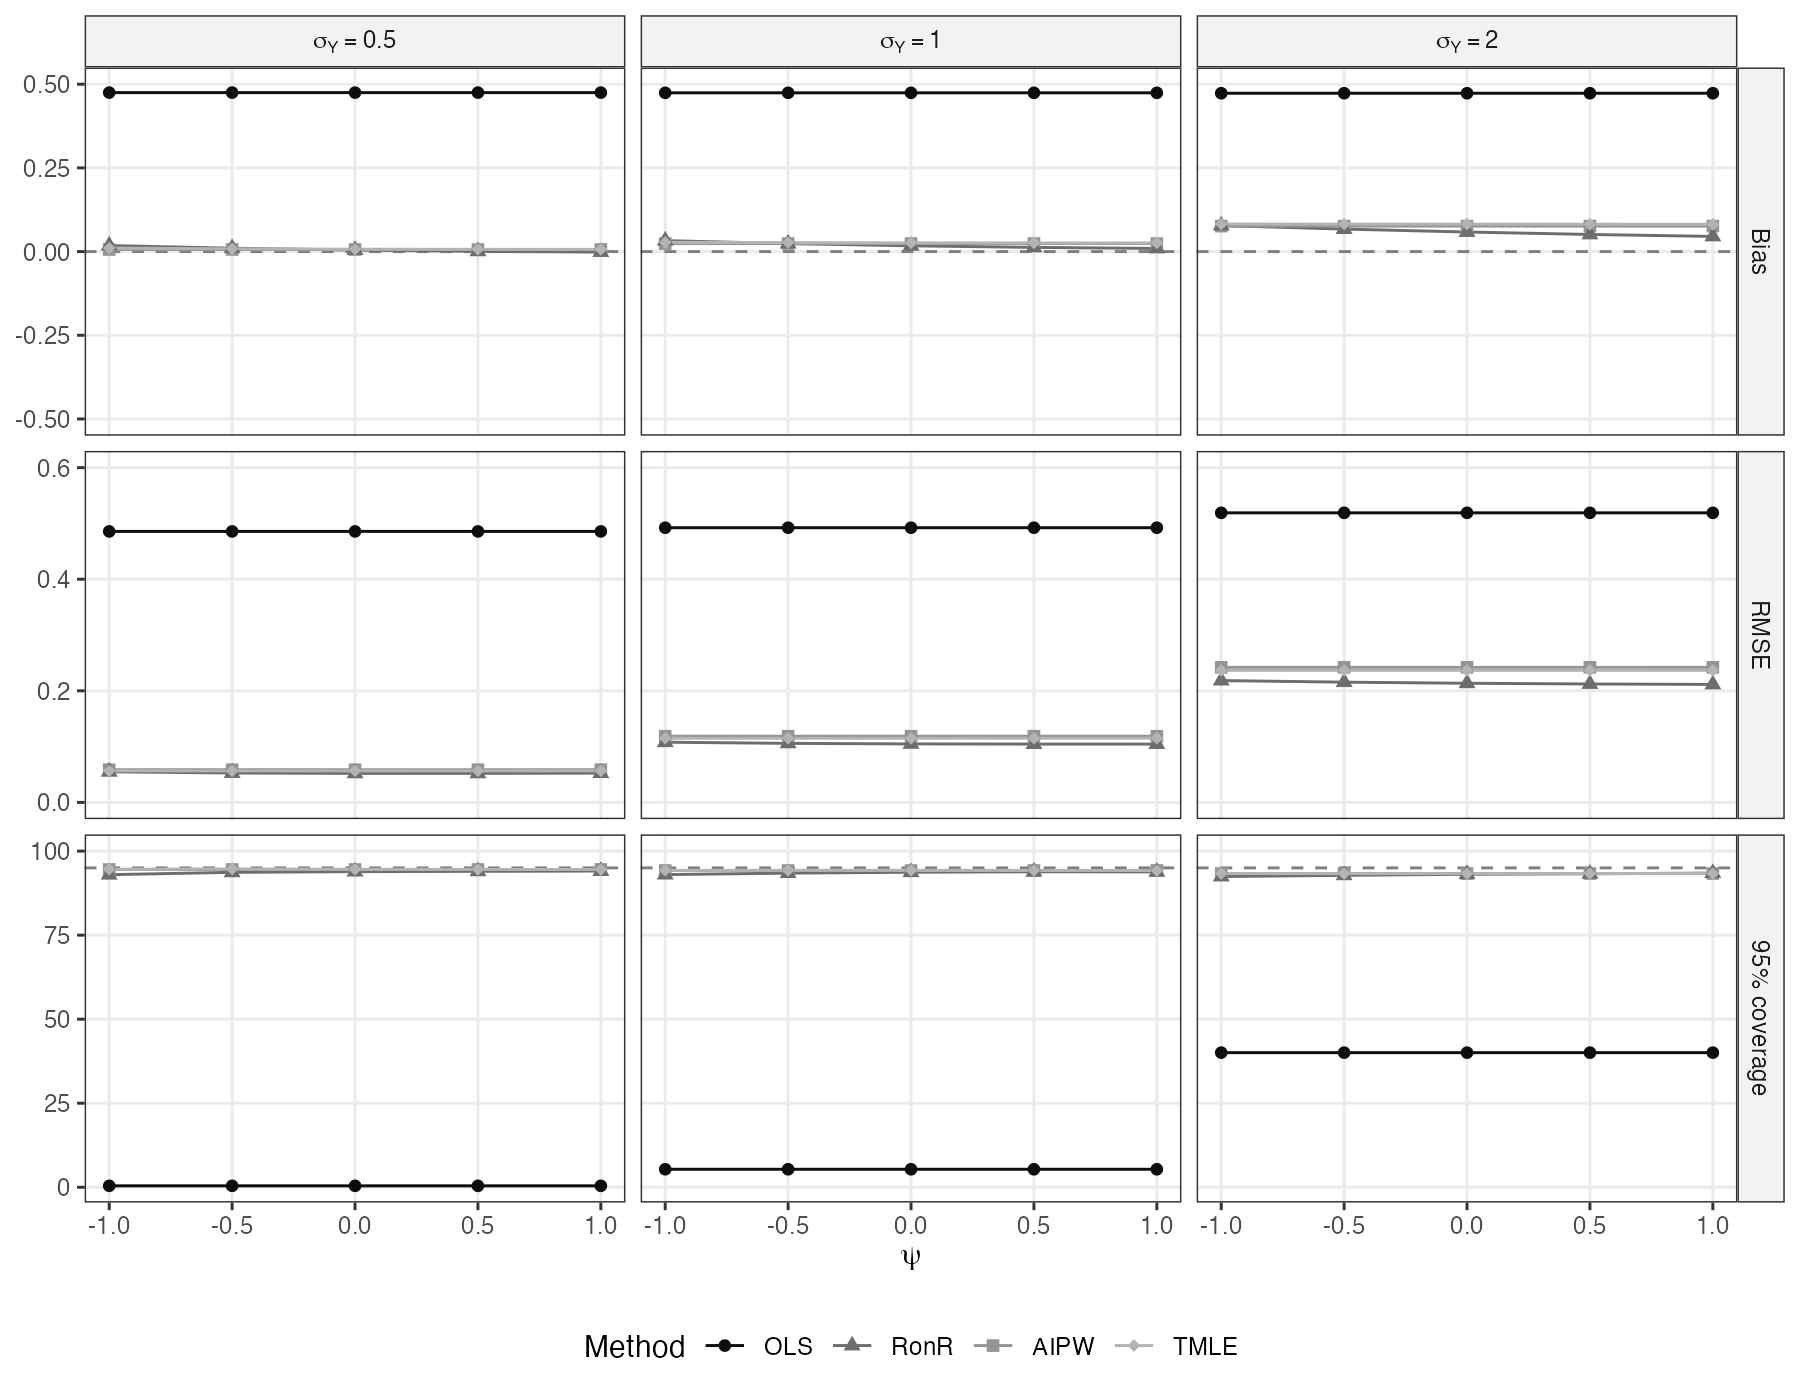
\includegraphics[width=\textwidth]{sim_performance_sl.png}
\caption{Finite-sample performance of residual-on-residual regression (RonR), augmented inverse probability weighting (AIPW), targeted maximum likelihood estimation (TMLE), and a naive linear-additive ordinary least squares (OLS) comparator across $10{,}000$ Monte Carlo replicates per scenario at $n = 500$. Rows display bias (top), root mean squared error (RMSE; middle), and empirical 95\% Wald confidence interval coverage (bottom). Columns correspond to the outcome error scale $\sigma_Y \in \{0.5, 1, 2\}$. The horizontal axis shows the true treatment effect $\psi \in \{-1, -0.5, 0, 0.5, 1\}$. Dashed reference lines indicate bias $= 0$ and 95\% coverage. Nuisance functions for RonR, AIPW, and TMLE were fit by a 5-fold cross-validated Super Learner over a library of four generalized linear model variants spanning main effects, two-way interactions, and quadratic terms for the continuous confounders.}
\label{fig:sim_performance}
\end{figure}

\section{Discussion}

Modern semiparametric theory has produced several closely related strategies for estimating an average treatment effect from observational data using machine learning to flexibly adjust for confounders. Residual-on-residual regression takes an alternative route compared to standard AIPW or TMLE, assuming a linear structure for the exposure-outcome relationship, but leaving all other variables coded in the outcome model nonparametrically specified. The causal effect of interesest is then estimated using a no-intercept OLS model that regresses outcome model residuals against exposure model residuals. If the partially linear model with a constant treatment effect holds, all three estimators target the same parameter (i.e., are asymptotically equivalent) and, under cross-fitting with appropriately fast nuisance convergence rates, are asymptotically linear with the same efficient influence function.\cite{Chen2026} 

Despite this asymptotic equivalence, residual-on-residual regression has practical advantages motivating its use alongside AIPW and TMLE. The closed-form coefficient and robust standard error make the estimator easy to implement in a wide variety of software platforms. Unlike AIPW and TMLE, the residual-on-residual estimator avoids explicit weighting by the propensity score ($1/\hat\pi(C)$ and $1/\{1 - \hat\pi(C)\}$), which translates into greater stability when some propensity scores approach 0 or 1. Vansteelandt and Sjolander emphasize this point in the context of the closely related g-estimation approach, noting that it requires only a model for the conditional expectation of the exposure (as opposed to its conditional density).\cite{VansteelandtSjolander2016} Because of its close relationship to g-estimation, the simplicity and stability of residual-on-residual regression makes it a natural triangulation tool: any disagreement between AIPW, TMLE, or residual-on-residual estimates points to potential model dependence that warrants further investigation.

The interpretability of residual-on-residual regression as an estimator of the average treatment effect, however, hinges on the assumption that the treatment effect is constant across the population. When this assumption is violated, the estimator continues to converge to a meaningful causal quantity. Lal and Chou recently show that with a binary exposure and heterogeneous unit-level effects $\theta_i$, the probability limit of residual-on-residual regression is a conditional variance-weighted average $\E[\omega_i \theta_i]$, with weights $\omega_i = (A_i - \pi(C_i))^2 / \E[(A_i - \pi(C_i))^2]$. This means that units whose propensity scores are closest to $0.5$ contribute most strongly, while units whose propensity scores are closer to the boundaries contribute less information to the estimator.\cite{LalChou2026} Thus, like g estimation, residual-on-residual regression is less sensitive to potential violations of the positivity assumption. 

However, the bias of the parameter estimate from a mis-specified residual-on-residual estimator relative to the true average treatment effect is exactly $\text{Cov}(\omega_i, \theta_i)$ and vanishes only when the treatment is assigned with constant probability across the population or when effects are homogeneous.\cite{LalChou2026} This insight was first highlighted  by Vansteelandt and Sjolander, who obtain the same conclusion within the structural nested mean model framework: when the constant-effect assumption is misspecified but the propensity is correctly modeled, the linear-SMM g-estimator (which is asymptotically equivalent to residual-on-residual regression) converges to $\E[\text{Var}(A \mid L) \, \{Y(1) - Y(0) \mid L\}] / \E[\text{Var}(A \mid L)]$, a variance-weighted average of conditional effects.\cite{VansteelandtSjolander2016} For continuous treatments with a nonlinear dose-response, Lal and Chou further show that the bias of residual-on-residual regression compounds with a curvature term, because the relevant marginal derivative is evaluated at a convex combination of the observed treatment and its conditional mean rather than at the observed treatment value itself.\cite{LalChou2026} AIPW and TMLE, which target the average treatment effect directly through the efficient influence function, do not share these biases.

These observations situate residual-on-residual regression within the broader family of g-estimators of structural nested mean models, of which the linear no-effect-modification structural nested mean model is the simplest member.\cite{VansteelandtSjolander2016} Robinson's residual-on-residual regression coincides asymptotically with the two-step g-estimator that (i) fits the propensity score $\pi(C)$ by regressing the exposure on $C$ and (ii) regresses the outcome on the centered exposure $A - \pi(C)$ with adjustment for $C$, yielding an estimator that is doubly robust against misspecification of either the propensity or the conditional outcome regression.\cite{VansteelandtSjolander2016} Recognizing residual-on-residual regression as a g-estimator of a constant-effect structural nested mean model clarifies both its strengths (double robustness, computational simplicity, and stability under near-positivity violations) and its limitations, notably that the constant-effect assumption is required to recover the average treatment effect, and that any effect modification by covariates must be encoded explicitly within the structural nested mean model to be recovered without bias.

Residual-on-residual regression also forms the foundation for several recent extensions to heterogeneous treatment effects. Notably, the R-learner generalizes the ``partialling-out'' idea to estimate conditional average treatment effects such as $\tau(C) = \E[Y(1) - Y(0) \mid C]$ by minimizing a regularized empirical version of a loss function very similar to the residual-on-residual regression approach, but over a flexible function class for $\tau$.\cite{Nie2021} Thus, while we demonstrate here it's use in the context of estimating average treatment effects encoded in a partially linear model, the approach can be adapted to estimate heterogeneous treatment effects, and effect modification. 

In the partially linear model with an approximately constant treatment effect, residual-on-residual regression delivers an interpretable, computationally efficient, and stable estimator of a treatment effects that complements AIPW and TMLE, and provides a natural triangulation strategy for observational causal inference. When the constant treatment effect assumption is suspect, residual-on-residual regression should be paired with an explicit assessment of effect heterogeneity, possibly through stratified analyses, estimation of conditional average treatment effects via the R- or other ``learners''.\cite{Kennedy2023} Overall, residual-on-residual regression, though underutilized, can be of benefit to researchers interested in estimating effects with machine learning. 

\newpage

\begin{table}[ht]
\centering
\caption{Adjusted risk difference (per 100 participants) for the association between periconceptional high vegetable intake ($\geq$ 1.25 cups per 1{,}000 kcal) and preeclampsia, estimated by residual-on-residual regression, augmented inverse probability weighting (AIPW), and targeted maximum likelihood estimation (TMLE) in the Nulliparous Pregnancy Outcomes Study: Monitoring Mothers-to-be Heart Health Study (nuMoM2b-HHS; $n = 7{,}923$). All estimators were fit with a 10-fold cross-fitted Super Learner ensemble, adjusting for sociodemographic, behavioral, medical, neighborhood, and dietary confounders. CL, confidence limit.} 
\label{tab:numom_results}
\begin{tabular}{lrrr}
  \toprule
Method & Risk Difference (per 100) & Lower 95\% CL & Upper 95\% CL \\ 
  \midrule
Residual-on-Residual & -1.52 & -2.98 & -0.07 \\
  AIPW & -1.06 & -2.87 & 0.74 \\
  TMLE & -1.73 & -3.58 & 0.11 \\
   \bottomrule
\end{tabular}
\end{table}

\newpage

\begin{figure}[ht]
\centering
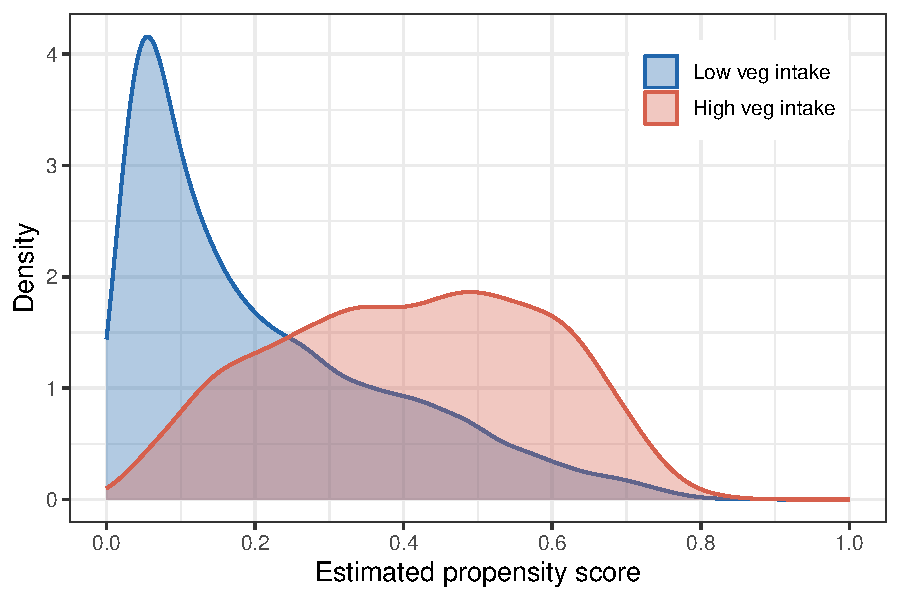
\includegraphics[width=0.75\textwidth]{ps_overlap.pdf}
\caption{Estimated propensity score distributions for the exposure (periconceptional high vegetable intake, $\geq$ 1.25 cups per 1{,}000 kcal) in the Nulliparous Pregnancy Outcomes Study: Monitoring Mothers-to-be Heart Health Study (nuMoM2b-HHS; $n = 7{,}923$). Propensity scores were estimated using a 10-fold cross-fitted Super Learner ensemble of the sample mean, generalized linear models, random forests (ranger), elastic net (glmnet), and multivariate adaptive regression splines (earth). Densities are shown separately for participants with low ($<$ 1.25 cups per 1{,}000 kcal) and high vegetable intake.}
\label{fig:ps_overlap}
\end{figure}

\newpage

\bibliographystyle{epid}
\bibliography{main_references}

\newpage

\appendix

\section{Simulation Study: Complete Implementation Details}\label{sec:sim_appendix}

This appendix provides a complete specification of the Monte Carlo simulation study reported in the Simulation Study and Simulation Results sections of the main paper. The full R replication code is in \texttt{code/simulation\_study\_sl.R} of the project's associated GitHub repository, which also contains the seed bank used and the script that produces Figure~\ref{fig:sim_performance}.

\subsection*{A.1\quad Data-generating mechanism}

For each Monte Carlo replicate we drew an independent and identically distributed sample of size $n = 500$ from the following joint distribution. The confounders $C_1$ and $C_2$ were independently drawn from a Uniform$(-1, 1)$ distribution, $C_3$ and $C_4$ from a standard Normal distribution, and $C_5$ and $C_6$ from independent Bernoulli distributions with success probabilities $0.4$ and $0.5$, respectively. The variable $C_6$ entered neither the propensity nor the outcome model and serves as a noise covariate. The binary exposure was drawn from $A_i \sim \mathrm{Bernoulli}\{\pi(C_i)\}$, where $\pi(C) = \expit\{\eta(C)\}$ and
$$\eta(C) = -0.3 + 0.9 C_1 + 1.0 C_1^2 - 0.7 C_2 + 0.8 C_2 C_3 - 0.5 C_3 + 0.6 C_5 - 0.4 C_5 C_4.$$
The continuous outcome was generated from a partially linear model:
$$Y_i = 125 + \psi A_i + g(C_i) + \varepsilon_i, \qquad \varepsilon_i \sim \mathcal{N}(0, \sigma_Y^2),$$
where
$$g(C) = 1.2 C_1 + 1.5 C_1^2 - 1.0 C_2 + 1.4 C_2 C_3 - 0.8 C_3 + 0.7 C_4 + 1.0 C_5 - 0.6 C_5 C_4.$$
Because $g$ does not interact with $A$, the population average treatment effect equals $\psi$ exactly. We swept $\psi \in \{-1, -0.5, 0, 0.5, 1\}$ crossed with $\sigma_Y \in \{0.5, 1, 2\}$, yielding 15 scenarios. The intercept of $125$ is cosmetic and affects neither bias nor coverage; it places the outcome on a scale resembling the application data.

\subsection*{A.2\quad Monte Carlo replication and common random numbers}

We performed $10{,}000$ Monte Carlo replicates per scenario. Seeds were taken from a fixed reproducible seed bank (\texttt{data/random\_seed\_values.csv}) and held fixed across scenarios so that contrasts between scenarios share Monte Carlo noise (common random numbers). The Monte Carlo standard error on the reported bias is therefore approximately the empirical standard error divided by $\sqrt{10{,}000} = 100$, which is small relative to the entries shown in Figure~\ref{fig:sim_performance}.

\subsection*{A.3\quad Nuisance estimation}

Within each replicate we estimated three nuisance functions: $\pi(C) = P(A = 1 \mid C)$, $\mu(A, C) = \E[Y \mid A, C]$, and $\nu(C) = \E[Y \mid C]$. Each was fit by \texttt{CV.SuperLearner} from the R package \texttt{SuperLearner} using a 5-fold outer cross-validation. The same outer-fold partition was shared across the three nuisance fits by passing identical \texttt{validRows} indices, ensuring cross-fitted predictions for all three nuisances are aligned by observation index. Within each outer training partition, ensemble weights were chosen by an inner 5-fold cross-validation using non-negative least squares (\texttt{SuperLearner}'s default for Gaussian outcomes; logistic for binary).

The Super Learner library comprised four generalized linear model variants:
\begin{enumerate}
\item \texttt{SL.glm}: main effects in the input columns only.
\item \texttt{SL.glm.interaction}: main effects plus all two-way interactions between input columns.
\item \texttt{SL.glm.quad}: main effects plus a quadratic term for each continuous column (identified at fit time as a numeric column with more than two unique values not all contained in $\{0,1\}$).
\item \texttt{SL.glm.full}: main effects, quadratic terms for the continuous columns, and all two-way interactions between the original input columns.
\end{enumerate}
Only \texttt{SL.glm.full} is correctly specified for the data-generating mechanism above. Including the simpler members forces the Super Learner to discover this empirically through inner cross-validation rather than by oracle assignment. For $\mu(A, C)$, the design matrix passed to each library member included $A$ as the first column; the interaction- and full-models therefore also estimate $A \cdot C$ interactions, which are zero in expectation by construction.

Counterfactual outcome predictions $\hat\mu_0(C_i)$ and $\hat\mu_1(C_i)$ were obtained by, for each outer fold $k$, predicting on the validation rows of fold $k$ with $A$ forced to $0$ and $1$ in turn, using the Super Learner ensemble trained on the remaining four folds. Predictions were stored by positional assignment so that observation ordering is preserved. The propensity-score predictions were truncated to $[0.01, 0.99]$ prior to use in any estimator.

\subsection*{A.4\quad Estimator implementations}

The four estimators reported in Figure~\ref{fig:sim_performance} were implemented as follows.
\begin{itemize}
\item \emph{Naive OLS comparator.} Fit by \texttt{lm(Y \textasciitilde~A + C1 + \ldots + C6)} on the simulated data, with the model-based standard error from \texttt{summary(fit)\$coefficients}. This estimator is deliberately misspecified relative to the data-generating mechanism (it omits $C_1^2$, $C_2 C_3$, and $C_5 C_4$).
\item \emph{Residual-on-residual regression.} Fit by no-intercept ordinary least squares of $\tilde Y = Y - \hat\nu(C)$ on $\tilde A = A - \hat\pi(C)$, with HC3 robust standard errors from the \texttt{sandwich} package.
\item \emph{AIPW.} Computed as the sample mean of the efficient influence function
$$\varphi(O; \hat\pi, \hat\mu) = \hat\mu_1(C) - \hat\mu_0(C) + \frac{A \{Y - \hat\mu_1(C)\}}{\hat\pi(C)} - \frac{(1 - A)\{Y - \hat\mu_0(C)\}}{1 - \hat\pi(C)},$$
with standard error equal to the sample standard deviation of $\varphi$ divided by $\sqrt{n}$.
\item \emph{TMLE.} Computed by the \texttt{tmle} R package with $\mathrm{family} = \texttt{"gaussian"}$, the cross-fitted initial outcome predictions supplied via $Q = (\hat\mu_0, \hat\mu_1)$, the cross-fitted truncated propensity supplied via $g_{1W} = \hat\pi$, and the standard error taken from the package's targeted influence-function variance.
\end{itemize}

\subsection*{A.5\quad Software and reproducibility}

All computation was performed in R using the \texttt{SuperLearner}, \texttt{tmle}, \texttt{sandwich}, \texttt{lmtest}, \texttt{future.apply}, and \texttt{progressr} packages. Replicates were parallelized across CPU cores using a \texttt{multisession} \texttt{future} plan with per-replicate seeding managed by \texttt{future.seed = TRUE}; this keeps draws within a replicate reproducible while allowing the work to be distributed. Per-replicate Super Learner ensemble weights for each of $\pi$, $\mu$, and $\nu$ were recorded alongside the point estimates and standard errors, supporting post hoc diagnosis of which library members the ensemble was relying on for each scenario. The complete simulation pipeline is contained in \texttt{code/simulation\_study\_sl.R}; the figure-producing block at the end of that script writes \texttt{output/figures/sim\_performance\_sl.png}, which is reproduced as Figure~\ref{fig:sim_performance} of the main paper.

\end{document}
